%
% @author   Shmish  "shmish90@gmail.com"
% @legal    MIT     "(c) Christopher Schmitt"
%


\documentclass{article}


%
% Document Imports
%

\usepackage{fancyhdr}
\usepackage{extramarks}
\usepackage{amsmath}
\usepackage{amssymb}
\usepackage{amsthm}
\usepackage{amsfonts}
\usepackage{algpseudocode}
\usepackage[table,xcdraw]{xcolor}
\usepackage{color}
\usepackage{tikz}
\usepackage{forest}
\usepackage{listings}
\usepackage{karnaugh-map}
\usepackage{graphicx}


\definecolor{dkgreen}{rgb}{0,0.6,0}
\definecolor{gray}{rgb}{0.5,0.5,0.5}
\definecolor{mauve}{rgb}{0.58,0,0.82}


\lstset{
  frame=tb,
  language=Verilog,
  aboveskip=3mm,
  belowskip=3mm,
  showstringspaces=false,
  columns=flexible,
  basicstyle=\ttfamily,
  numbers=none,
  numberstyle=\tiny\color{gray},
  keywordstyle=\color{blue},
  commentstyle=\color{dkgreen},
  stringstyle=\color{mauve},
  breaklines=true,
  breakatwhitespace=true,
  tabsize=3
}


%
% Document Configuation
%

\newcommand{\hwAuthor}{Christopher Schmitt}
\newcommand{\hwSubject}{CS 354}
\newcommand{\hwSection}{Section 02}
\newcommand{\hwSemester}{Fall 2019}
\newcommand{\hwAssignment}{Assignment 2}


%
% Document Enviornments
%

\setlength{\headheight}{65pt}
\pagestyle{fancy}
\lhead{\hwAuthor}
\rhead{
  \hwSubject \\
  \hwSection \\
  \hwSemester \\
  \hwAssignment
}

\newenvironment{problem}[1]{
  \nobreak\section*{Problem #1}
}{}


%
% Document Start
%

\begin{document}
  \begin{problem}{1}
    This simple ALU supports five functions: AND, OR, ADD, SUB, and SLT.  This
    ALU can be simplified by using the fact that in a 2's complement scheme, the
    SUB operation can be achived by inverting the right hand, adding one, and
    then performing standard addition.  The four-bit ALU is created by instantiating
    four one-bit ALUs.  The design of the one bit ALU is very simple.  It is created
    by instantiating an AND gate, an OR gate, an adder, and a buffer.  All these
    operations are performed in parallel.  The least two significant bits on the
    opcode line drives a 4x1 multiplexer which selects one of these computations
    and puts it on the result line.  The effect of chaining four of these ALUs
    together is a four-bit ALU.  The final ALU in the chain of four has some extra
    functions, namely, overflow detetion and driving the `set` line.  Overflow
    detection is achived by handling two unique cases (The sign of the operands do
    not match the sign of the output).  In order to limit overflow detection to
    arithmetic operations (disabled for logical ops), the overflow line is ANDed with
    the second bit of the opcode (which is always 1 when the operation is arithmetic).

    \begin{center}
      \lstinputlisting{src/ALU.v}
    \end{center}

    \begin{center}
      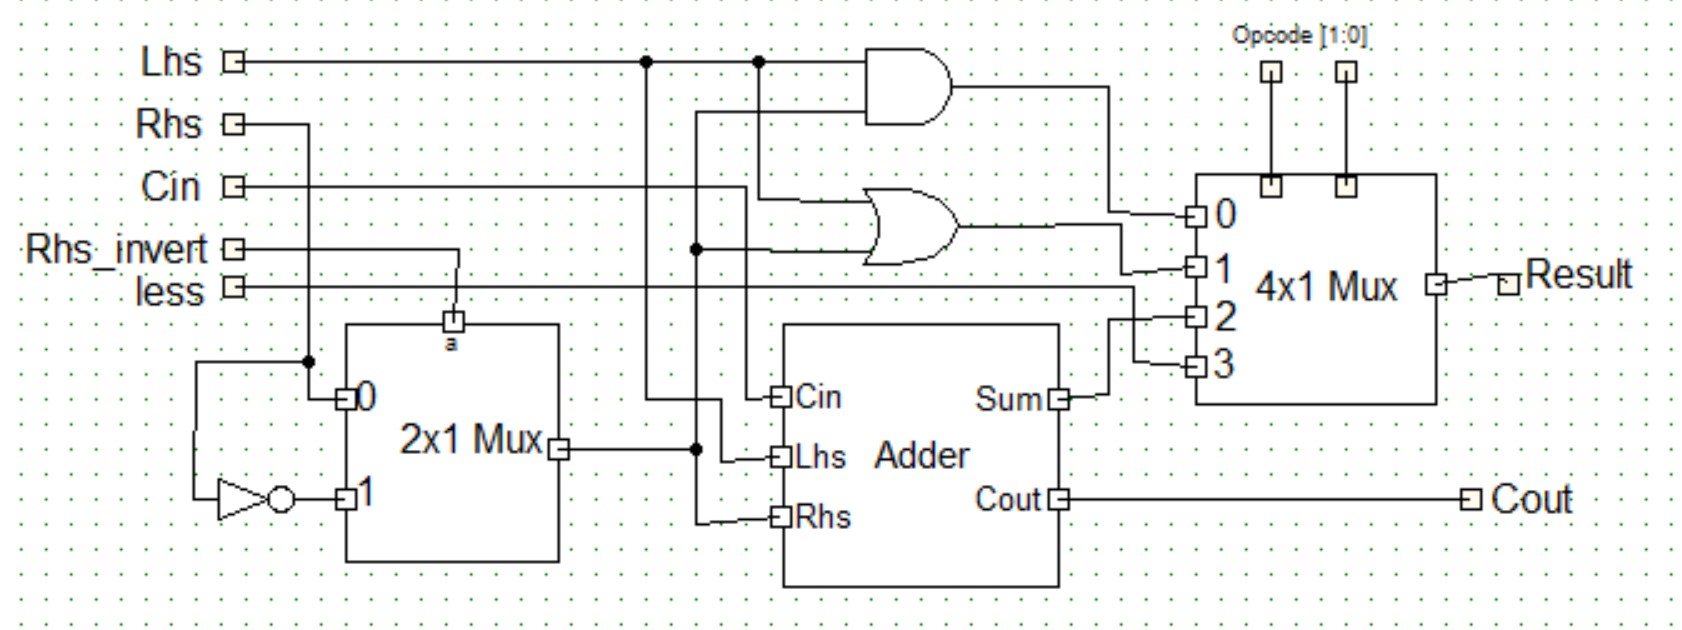
\includegraphics[scale=0.65]{images/OneBitALU.jpg}
      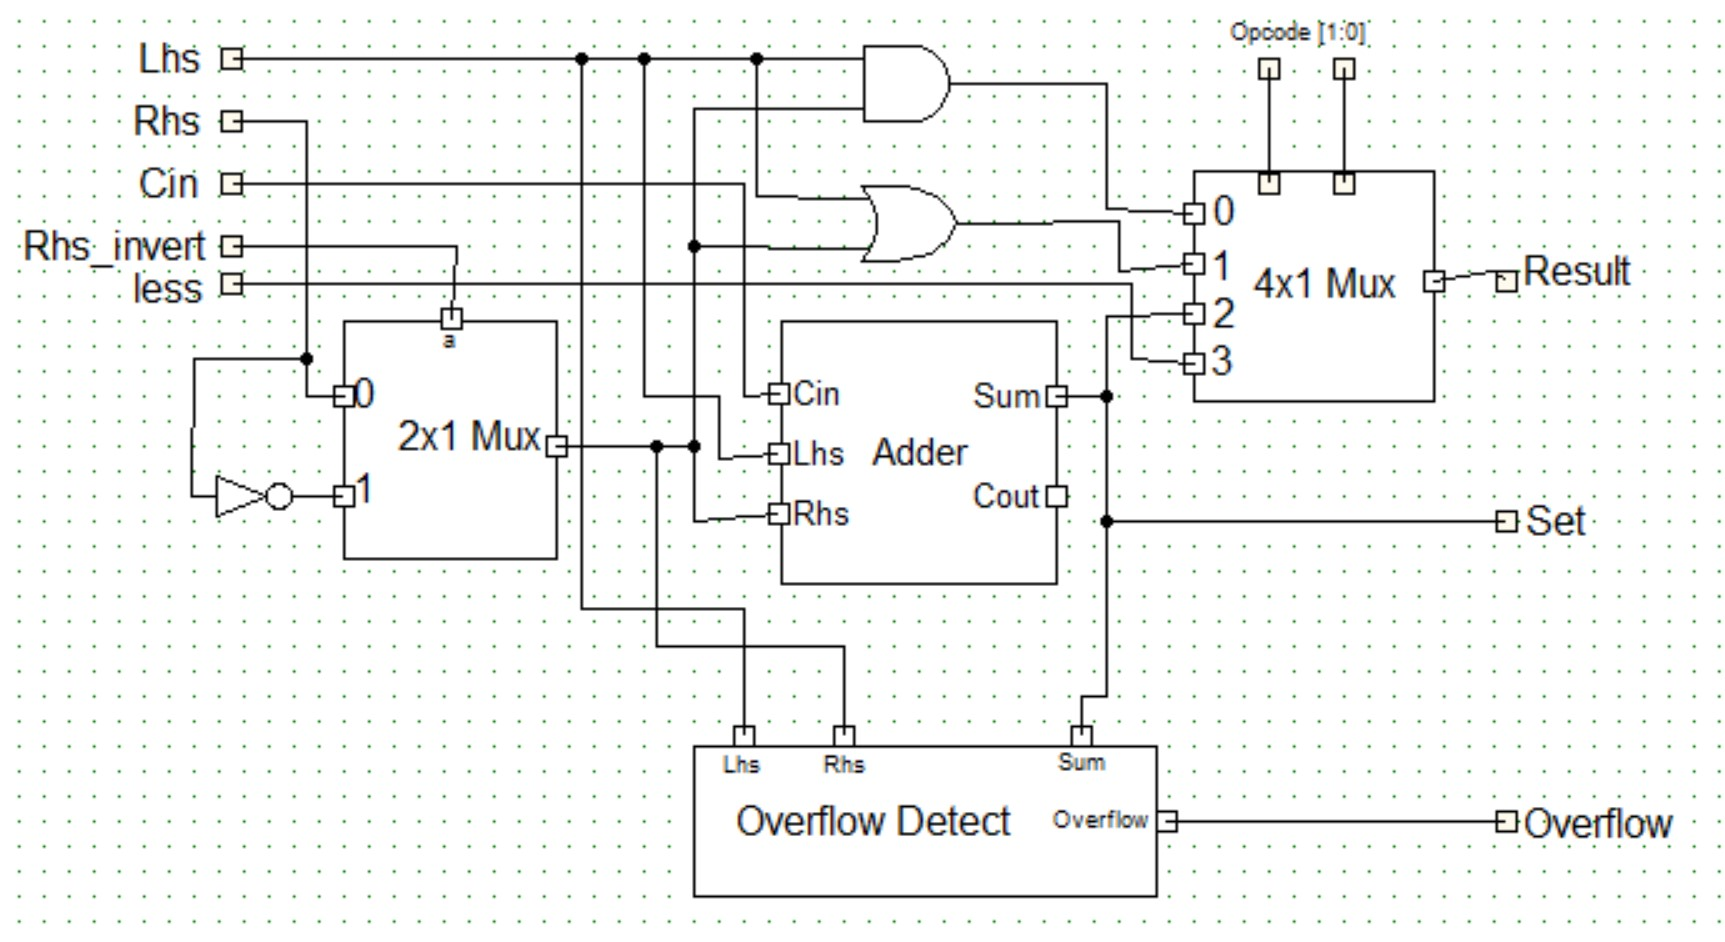
\includegraphics[scale=0.65]{images/OneBitALU_Set.jpg}
      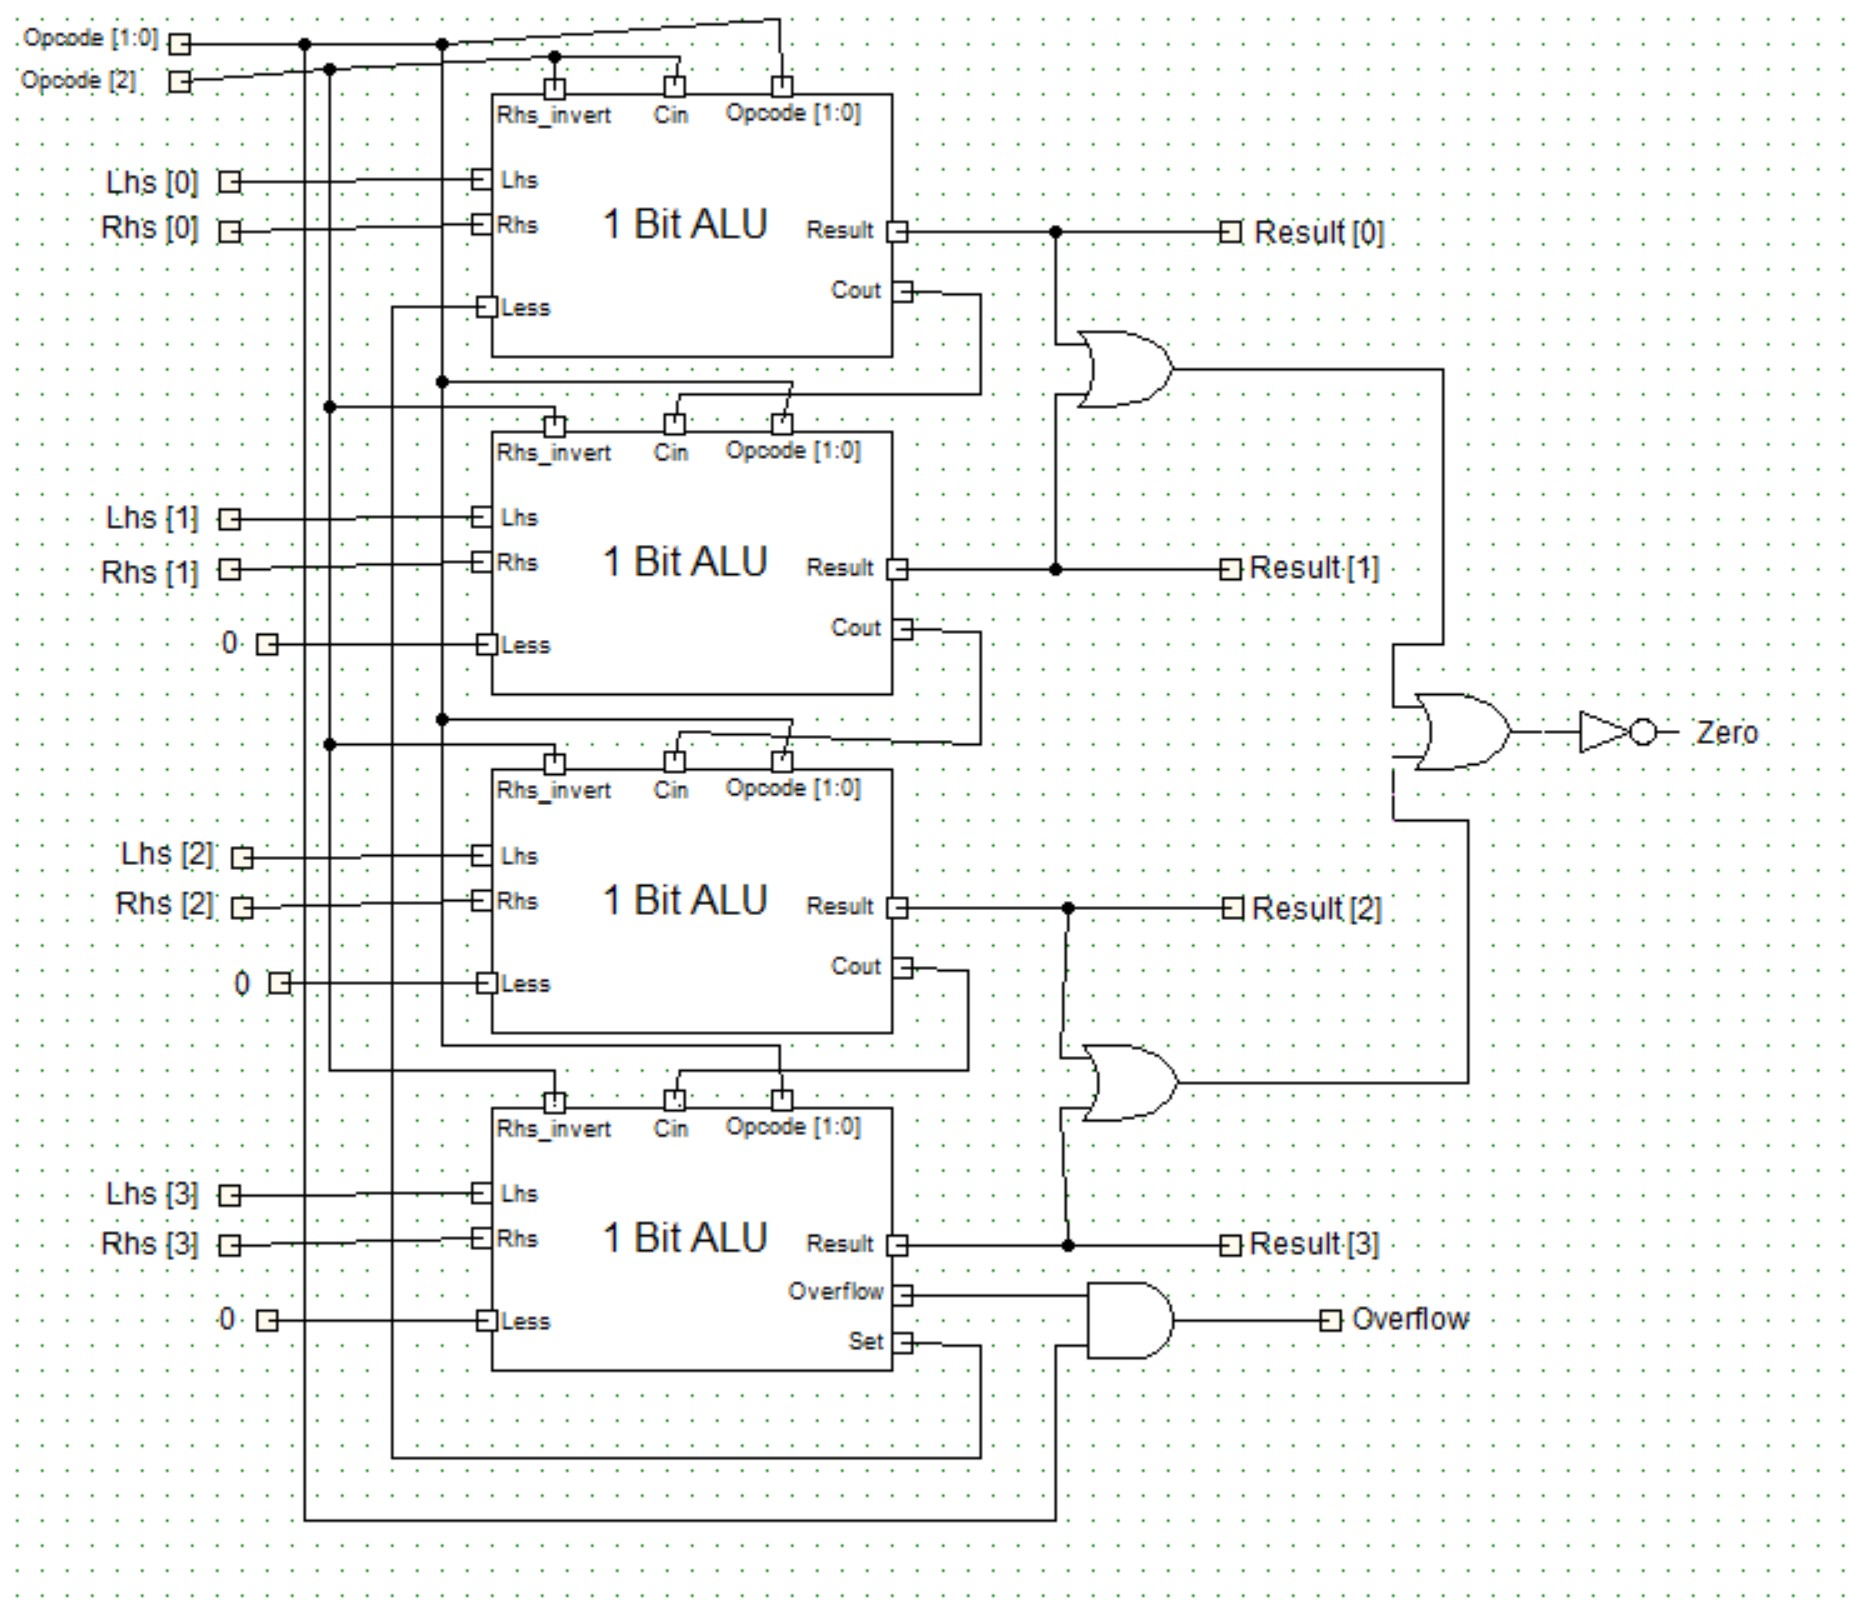
\includegraphics[scale=0.5]{images/ALU.jpg}
    \end{center}

    \begin{center}
      \begin{lstlisting}
        D:\School\CS-354>vvp a.out
        operation  lhs      rhs      result   overflow  zero
        2 010      2 0010   2 0010   4 0100   0         0
        2 010      4 0100   1 0001   5 0101   0         0
        2 010      6 0110   6 0110  -4 1100   1         0
        2 010      1 0001   1 0001   2 0010   0         0
        2 010      7 0111  -7 1001   0 0000   0         1
        6 110      5 0101   2 0010   3 0011   0         0
        6 110      5 0101   7 0111  -2 1110   0         0
        6 110     -6 1010  -6 1010   0 0000   0         1
        6 110     -7 1001   7 0111   2 0010   1         0
        6 110      2 0010  -2 1110   4 0100   0         0
        0 000     -1 1111   3 0011   3 0011   0         0
        0 000     -1 1111  -1 1111  -1 1111   0         0
        0 000      3 0011  -4 1100   0 0000   0         1
        1 001      0 0000   1 0001   1 0001   0         0
        1 001      0 0000   3 0011   3 0011   0         0
        1 001     -1 1111  -1 1111  -1 1111   0         0
        7 111      3 0011   3 0011   0 0000   0         1
        7 111      3 0011   2 0010   0 0000   0         1
        7 111      2 0010   3 0011   1 0001   0         0
      \end{lstlisting}
    \end{center}
  \end{problem}
\end{document}